
\section{Convergence of Sequences}

\subsection{Intuitive and Formal Definitions}\label{convseq}

Consider the sequence $a_n=\frac{1}{2^n}$.  Listing out a few terms, we see that $a_n$ looks like:
$$1,\frac{1}{2},\frac{1}{4},\frac{1}{8},\frac{1}{16},\ldots$$

We would like a way to describe the long-term behavior of such a sequence.  Intuitively, we see that the numbers are becoming arbitrarily close to zero. 

\begin{exercise}{The Idea of Convergence \Coffeecup}
\begin{itemize}
\item Label the $y$ coordinates on the graph of the sequence below.

	\begin{center}
	\includegraphics[width=200pt,height=75pt]{ChapterSeqSer/Figures/convergence1tenth.eps}
	\end{center}

\item How far into the sequence would you have to travel to find only terms that are no more than one-tenth from zero?  That is to say, how large does $n$ have to be to guarantee that $a_n$ is between one-tenth and zero?
\solushun{
The $4^{\text{th}}$ term gets us below one-tenth.\\
}{1in}
\item How far into the sequence would you have to travel to find only terms that are no more than one-hundredth from zero?
\solushun{
We want $x$ such that $2^x \geq 100$. Since $2^7=128$ we need 7 terms.\\
}{1in}
\item How far into the sequence would you have to travel to find only terms that are no more than  one-thousandth from zero?
\solushun{By the same reasoning as above, we can go out to 10 terms, since $2^{10}=1024\geq 1000$.\\}{1in}
\end{itemize}
\end{exercise}

No matter how small of a measurement we choose (one-tenth, one-hundredth, one-thousandth, etc), we could always find that after a certain point, all of our sequence terms are no further than that measurement from zero.  This is exactly the notion we will reformulate in a more formal manner to define sequential convergence.  

  Recall the mathematical shorthands often used to help concisely state messy definitions: the symbol ``$\forall$'' means ``for all'' and the symbol ``$\exists$'' means ``there exists''.  See Chapter \ref{Overview} for more detail.  Also recall that for any real numbers $a$ and $b$, the distance between $a$ and $b$ can be written as $\left|a-b\right|$.  Using these shorthands, we \Nepsilonproof{define} the limit of a sequence!

\begin{definition}{Convergence of a Sequence}
We say the \conv{sequence} $a_n$ converges to a limit $L\in \mathbb{R}$ and write
$$\lim_{n \rightarrow \infty }a_n=L $$ if and only if$$\forall\epsilon>0, \exists N \in \mathbb{R}, \forall n\in \mathbb{N}, n>N \implies \left| a_n-L\right|<\epsilon$$ If no such $L$ exists, we say the \divergence{sequence} \emph{diverges}.
\end{definition}

	\begin{center}
	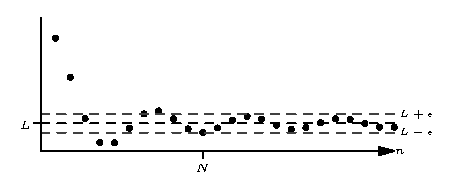
\includegraphics[width=400pt]{ChapterSeqSer/Figures/convergepsilon.eps}
	\end{center}

\begin{exercise}{Digesting the Definition \Coffeecup \Coffeecup}
\begin{itemize}
\item In the definition of convergence, what role does $\epsilon$ play?   Specifically, what is it bounding the distance between?
\solushun{
$\epsilon$ acts a a margin of error around the target value.\\
}{.5in}
\item In the definition of convergence, what role does $N$ play?  What role does $n$ play?
\solushun{
$N$ is acting like a cutoff value, above which the sequence should behave the way we want it to.\\
}{.5in}
\item Restate the formal definition of sequential convergence in words rather than symbols.  The statement 
$$ \lim_{n \rightarrow \infty } a_n = L $$ means...
\solushun{
As $n$ gets very large, or rather, as we go farther into the sequence, the terms get closer to our target value, $L$.
}{1in}
\end{itemize}
\end{exercise}


\begin{exercise}{The Fibonacci Numbers \Coffeecup \Coffeecup}\label{Fibbies}
Define the sequence of \seq{Fibonacci numbers} $F_n$ via the following \fibonacci{recursive formula}:
\begin{align*}
 F_0 &= 0 \\
 F_1 &= 1 \\
 F_n &=F_{n-1}+F_{n-2}
\end{align*}
\begin{itemize}

\item Compute the first eight terms of the Fibonacci sequence using the above recursion.  That is, compute $F_0$ through $F_7$. 

\solushun{
\begin{align*}
    F_0 &= 0\\
    F_1 &= 1\\
    F_2 &= F_0 + F_1 = 0+1 = 1\\
    F_3 &= F_1 + F_2 = 1+1 = 2\\
    F_4 &= F_2 + F_3 = 1+2 = 3\\
    F_5 &= F_3 + F_4 = 2+3 = 5\\
    F_6 &= F_4 + F_5 = 3+5 = 8\\
    F_7 &= F_5 + F_4 = 5+8 = 13\\
\end{align*}
}{2in}

\item Compute the following quantities:
\begin{align*}
F_2/F_1&=\\
F_3/F_2&=\\
F_4/F_3&=\\
F_5/F_4&=\\
F_6/F_5&=\\
F_7/F_6&=\\
\end{align*}

\solushun{
\begin{align*}
F_2/F_1&=\frac{1}{1}=1\\
F_3/F_2&=\frac{2}{1}=2\\
F_4/F_3&=\frac{3}{2}=1.5\\
F_5/F_4&=\frac{5}{3}=1.\overline{6}\\
F_6/F_5&=\frac{8}{5}=1.6\\
F_7/F_6&=\frac{13}{8}=1.625\\
\end{align*}
}{0in}

\item What would you conjecture about $$\lim_{n \rightarrow \infty} F_{n+1}/F_n$$ Does it seem to be going to infinity, zero, or stabilizing at something inbetween?
\solushun{
It seems to be stabilizing at some value around $1.62$. In actuality, it converges to the Golden Ratio: $1.61803\ldots$.\\
}{1in}
\end{itemize}

\end{exercise}

It is difficult to tell exactly what that limit of ratios is without knowing an explicit formula for the Fibonacci numbers.  Stay tuned, as we will find this in a later chapter!  

\begin{exercise}{Comparing Growth Orders of Sequences \Coffeecup \Coffeecup }
Rank the following functions in growth order from smallest to largest: \begin{align*}
a_n&=n^n \\
b_n&=e^n \\
c_n&=n^2 \\
d_n&=n!
\end{align*}

Note that for sequences we can compare growth orders in the same manner as we did in Subsection \ref{tomato}.  To compare the growth orders of two sequences $a_n$ and $b_n$, we compute $\lim_{n\to \infty} \frac{a_n}{b_n}$ and conclude that $a_n$ has larger growth order if the limit is infinity, $b_n$ has larger growth order if the limit is zero, and the growth orders are the same if the limit is a nonzero constant. Here you will need Stirling's Formula from Subsection \ref{Stirling}.
\solushun{In the context of computing limits, Stirling's Formula for factorials lets us use $n!\sim\sqrt{2\pi n} \left( \frac{n}{e} \right)^n$. Then we just need to compare the various expressions to each other.

\begin{align*}
c_n&=n^2 \\
b_n&=e^n \\
d_n&=n! \\
a_n&=n^n
\end{align*}}{2in}
\AnswerKeyEntry{In the context of computing a limit to infinity, it is fine to replace $n!$ by $\sqrt{2\pi n} \left( \frac{n}{e} \right)^n$.  Setting up limits of ratios and testing growth order with LHR and good old algebra will then verify that the order goes $n^2,e^n,n!,n^n$.}
\end{exercise}


\subsection{$N-\epsilon$ Proofs}

This complicated definition can be unwound into a to-do list for what one must do to prove that a sequence converges to a particular limit.  In particular, to show that the limit of $a_n$ is equal to a number $L$, one must:

\begin{itemize}
\item Let $\epsilon$ be an arbitrary positive real number.  
\item Choose $N$, typically defined as a function of $\epsilon$, since smaller values of $\epsilon$ will usually require a larger $N$ to be chosen. 
\item Let $n$ represent an arbitrary natural number greater than $N$.  
\item Using the definition of $N$ and the assumption that $n>N$, prove that any corresponding $a_n$ satisfies $\left|a_n-L\right|<\epsilon.$
\end{itemize}

Figuring out exactly what $N$ should be in terms of $\epsilon$ usually requires a bit of algebra before the proof is written up.  If the formula for $a_n$ is clean enough, you might be able to just work backwards from the inequality $\left| a_n-L \right|<\epsilon$.  If you solve it for $n$, you will find an expression that $n$ must be larger than.  Note here we are essentially just finding an inverse function for $a_n$.

\begin{example}{Solving for $N$}
Let us solve for $N$ with regards to our sequence $a_n=\frac{1}{2^n}$.  Since here we suspect $L=0$, we solve for $n$ in the following inequality: \begin{align*}
 \left| \frac{1}{2^n}-0 \right|&<\epsilon \\
  \frac{1}{2^n}&<\epsilon \\
  \frac{1}{\epsilon}&<2^n \\
  \ln\left(\frac{1}{\epsilon}\right)&<\ln\left(2^n\right) \\
  \ln\left(\frac{1}{\epsilon}\right)&<n\ln\left(2\right) \\
  \frac{\ln\left(\frac{1}{\epsilon}\right)}{\ln\left(2\right)}&<n \\
\end{align*}
Thus we determined our choice of $N$, namely $$N= \frac{\ln\left(\frac{1}{\epsilon}\right)}{\ln\left(2\right)}.$$
\end{example}

\begin{exercise}{Justifying Our Work \Coffeecup}
In words, annotate the above example to indicate why each line follows from the previous.
\end{exercise}

Now that we found our value for $N$, we are ready to follow the steps described above and construct our proof.

\begin{example}{\Nepsilonproof{Writing} an $N-\epsilon$ Proof}
Prove that $$\lim_{n\rightarrow \infty}\frac{1}{2^n}=0 $$
\begin{proof}
Let $\epsilon$ be an arbitrary positive real number.  Choose $N=\frac{\ln\left(\frac{1}{\epsilon}\right)}{\ln\left(2\right)}$.  Let $n$ be a natural number such that $n>N$.  Under these circumstances, we wish to show that a corresponding $a_n$ will be less than $\epsilon$ away from $0$.  Proceeding:

\begin{align*}
\left|\frac{1}{2^n}-0\right|&=\frac{1}{2^n} \\
&<\frac{1}{2^N} \\
&=\frac{1}{2^{\left(\frac{\ln\left(\frac{1}{\epsilon}\right)}{\ln\left(2\right)}\right)}} \\
&=\frac{1}{2^{\left(\log_2\left(\frac{1}{\epsilon}\right)\right)}} \\
&=\frac{1}{\frac{1}{\epsilon}} \\
&=\epsilon.
\end{align*}
Thus, for indices $n$ that are larger than our choice of $N$, the corresponding terms in our sequence are less than $\epsilon$ away from zero as desired.
\end{proof}
\end{example}

\begin{exercise}{Justifying Our Work \Coffeecup}
Once again in words, annotate the above example to indicate why each line follows from the previous.  Pay particular attention to identify where we used the starting assumption that $n>N$.
\end{exercise}

As this course does not go through a general treatment of what constitutes a proof or how to come up with one, the example above could be taken as a template for how an $N-\epsilon$ proof should be written.  In a more in-depth study of analysis, you will encounter more complicated situations where the above template may be too simplistic.  It will be expanded upon when you have the right tools!  For now, follow the above proof template for the following exercises:

\begin{exercise}{Verifying a Limit \Coffeecup \Coffeecup \Coffeecup}
Consider the sequence given by the following explicit formula: $$ a_n=\frac{2n}{n+1}$$
\begin{itemize}
\item List the terms of the sequence corresponding to $n=1$, $n=10$, $n=100$, and $n=1000$.  What do the terms appear to be converging to as $n$ goes to $\infty$?
\vspace*{1in}
\item If you choose $\epsilon=0.1$, what could the corresponding $N$ be?
\vspace*{1in}
\item If you choose $\epsilon=0.01$, what could the corresponding $N$ be? 
\vspace*{1in}
\item  Write an $N-\epsilon$ proof that verifies your guess above is correct.
\vspace*{3in}
\end{itemize}
\end{exercise}

\begin{exercise}{Writing $N-\epsilon$ Proofs \Coffeecup \Coffeecup \Coffeecup}
Write $N- \epsilon$ proofs for each of the following limits:

\begin{itemize}

\item $ \lim_{n \rightarrow \infty } \frac{n}{3n+1} = \frac{1}{3} $

\vspace*{3in}
\item $ \lim_{n \rightarrow \infty } \sqrt{9+1/n} = 3 $ 
\vspace*{3in}

\end{itemize}
\end{exercise}
